\subsection{Foam vs. Solid: Exploring Coaxial Cable Differences!}

\begin{tcolorbox}[colback=gray!10, colframe=black, title=E9F08] Which of the following is a significant difference between foam dielectric coaxial cable and solid dielectric coaxial cable, assuming all other parameters are the same? 
\begin{enumerate}[label=\Alph*)]
    \item A: Foam dielectric coaxial cable has lower safe maximum operating voltage
    \item B: Foam dielectric coaxial cable has lower loss per unit of length
    \item C: Foam dielectric coaxial cable has higher velocity factor
    \item \textbf{D: All these choices are correct}
\end{enumerate} \end{tcolorbox}

\subsubsection{Related Concepts}

To understand the differences between foam dielectric coaxial cable and solid dielectric coaxial cable, it is essential to grasp the following concepts:

1. \textbf{Dielectric Materials:}: Dielectric materials are insulators that can be polarized by an electric field. They are crucial in coaxial cables, as they separate the inner conductor from the outer conductor and influence the performance of the cable.

2. \textbf{Velocity Factor:}: The velocity factor (VF) of a cable describes how fast a signal travels through it compared to the speed of light in vacuum. A higher velocity factor indicates that the signal can travel faster, which is desirable in many applications.

3. \textbf{Loss per Unit Length:}: This refers to the signal attenuation as it propagates through the cable. Lower loss is typically preferable, as it allows the signal to maintain more power over longer distances.

4. \textbf{Operating Voltage:}: The safe maximum operating voltage indicates the upper limit of voltage that a cable can withstand without breaking down or allowing current to flow through the dielectric.

Given the question and the correct answer (D), we conclude that each of the statements about foam dielectric cables holds. To elaborate:

- \textbf{Foam dielectric coaxial cable has lower safe maximum operating voltage:}: Foam dielectrics can have lower breakdown voltages compared to solid dielectrics due to their structure and material properties.
  
- \textbf{Foam dielectric coaxial cable has lower loss per unit of length:}: Foam materials tend to offer lower attenuation, making them more efficient for signal transmission.

- \textbf{Foam dielectric coaxial cable has higher velocity factor:}: The reduced dielectric constant of foam relative to solid dielectrics results in a higher velocity factor.

Hence, all the mentioned choices about the properties of foam dielectric coaxial cable pertain to its significant differences from solid dielectric coaxial cable.

\subsubsection{Calculation Example}

While no specific calculations are needed for answering this question directly, one may find it valuable to understand how the velocity factor is determined using the dielectric properties:

\[
VF = \frac{1}{\sqrt{\epsilon_r}}
\]
where \(\epsilon_r\) is the relative permittivity of the dielectric material. For example, if the foam dielectric has a relative permittivity of 2.25, the velocity factor would be calculated as follows:

\[
VF = \frac{1}{\sqrt{2.25}} = \frac{1}{1.5} \approx 0.67
\]

\subsubsection{Diagram}

Here, a simple schematic can visualize the differences between foam and solid dielectric coaxial cables:

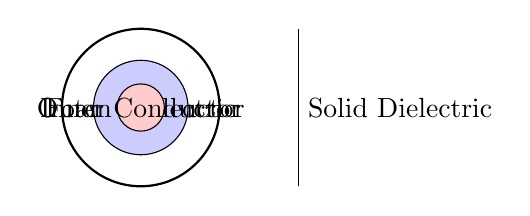
\begin{tikzpicture}
    \draw[thick] (0,0) circle(1) node {Outer Conductor};
    \draw[fill=blue!20] (0,0) circle(0.6) node {Foam Dielectric};
    \draw[fill=red!20] (0,0) circle(0.3) node {Inner Conductor};
    
    \draw[-] (2, -1) -- (2, 1) node[midway,right] {Solid Dielectric};
\end{tikzpicture}
